\section{Características del Dataset}

El dataset provisto por la cátedra contiene información sobre órdenes de compra, clientes, categorías, productos y reseñas de lo que podría ser una tienda en línea. \\
Al hacer varias consultas y visualizar los resultados se puede deducir que los datos no son reales, sino que son simulados. 
Por ejemplo, los nombres y apellidos de los clientes son muy genéricos y repetitivos, los nombres de los productos parecen ser palabras aleatorias sin significado, las ciudades tienen nombres inventados, las direcciones tienen estados y códigos postales de Estados Unidos pero países diferentes, etc. También aparecen valores sin sentido para algunos motivos de movimiento de inventario, como por ejemplo `Theft' o `Damage', pueden aparecer con valores positivos o negativos, lo carece de sentido real.

Además de esto, al realizar las consultas se encuentra con que los resultados son considerablemente uniformes, lo que refuerza la idea de que los datos son simulados. Esto es una lástima, pues dificulta la realización de análisis más profundos y la obtención de conclusiones interesantes.

A continuación muestro algunos gráficos que ilustran estas características simuladas o uniformes para las tablas \texttt{orders}, \texttt{customers} e \texttt{inventory\_logs}. Todas las consultas y gráficos de esta sección pueden encontrarse en el notebook \href{https://github.com/patricioibar/datos-tp1/blob/main/datos_uniformes.ipynb}{\texttt{datos\_uniformes.ipynb}}.

\subsection{Usuarios}
Para empezar, podemos ver en la figura \ref{fig:usuarios_por_pais} la cantidad de usuarios por país. Se puede observar que en todos los paises hay una cantidad muy similar de usuarios, y aún más, hay una cantidad también similar de usuarios sin país determinado. Esto es poco realista, ya que en la vida real la distribución de usuarios por país suele ser muy desigual debido a cuestiones socioeconómicas o poblacionales.
\begin{figure}[H]
    \centering
    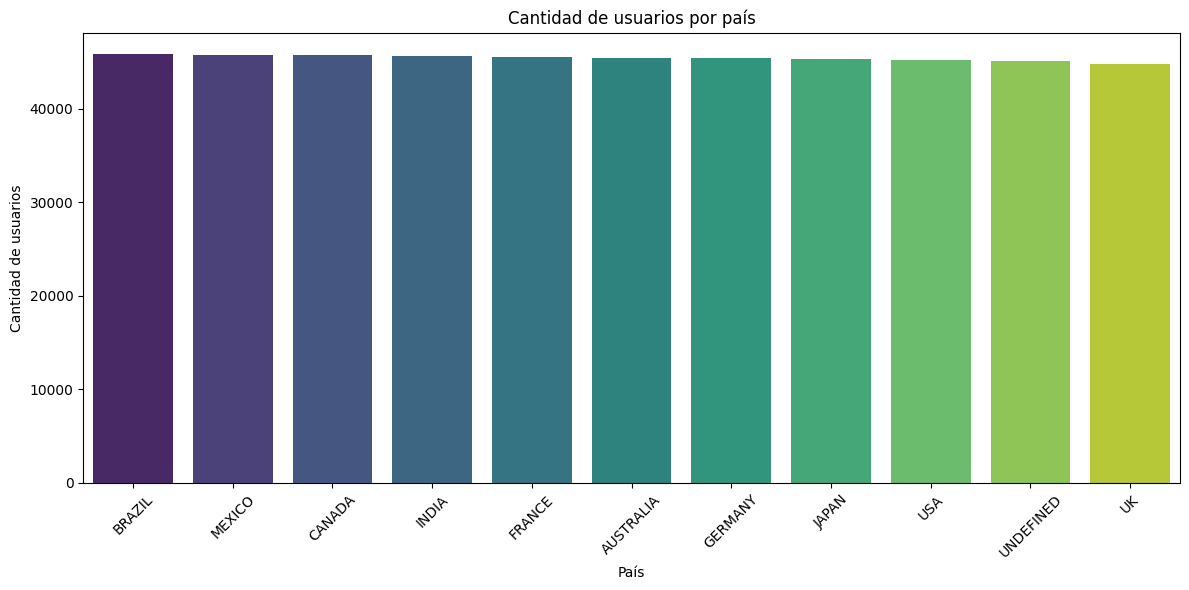
\includegraphics[width=0.8\textwidth]{imagenes/datos_uniformes/usuarios_por_pais.png}
    \caption{Cantidad de usuarios por país}
    \label{fig:usuarios_por_pais}
\end{figure}

En las siguientes dos figuras, podemos ver ilustrados los nuevos usuarios que se registran cada mes, diferenciados según el segmento al que pertenecen.
En estos gráficos se puede observar que, si bien no hay una cantidad exactamente igual de usuarios nuevos cada mes, la diferencia es muy pequeña. La mayor diferencia de nuevos usuarios está en el primer mes y el último mes registrado (ver figura \ref{fig:usuarios_nuevos_por_segmento_y_mes_de_registro}), sin embargo la proporción de nuevos usuarios respecto al total de usuarios sigue siendo muy similar en todos los meses (ver figura \ref{fig:proporcion_de_nuevos_usuarios}).

Otra cosa que se puede observar en estos gráficos es que la mayoría de los usuarios pertenecen al segmento \texttt{Regular}, mientras que los segmentos \texttt{Premium} y \texttt{Budget} son tienen menor volumen. Aún así, es destacable la proporción casi idéntica en estos últimos dos segmentos.

\begin{figure}[H]
    \centering
    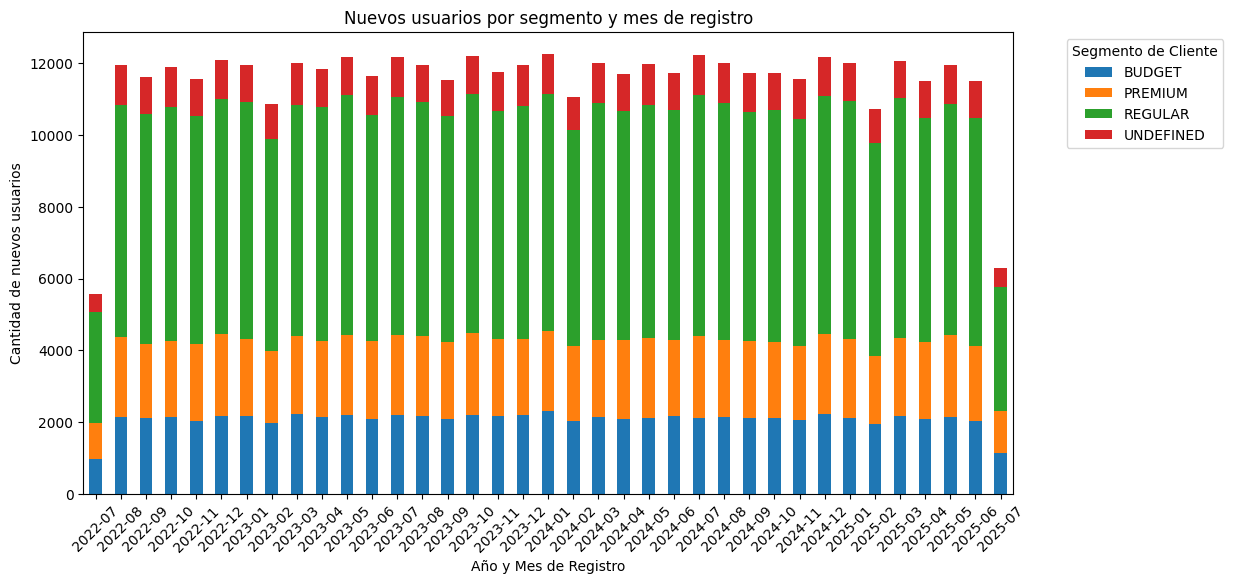
\includegraphics[width=0.8\textwidth]{imagenes/datos_uniformes/usuarios_nuevos_por_segmento_y_mes_de_registro.png}
    \caption{Cantidad de usuarios nuevos por segmento y mes de registro}
    \label{fig:usuarios_nuevos_por_segmento_y_mes_de_registro}
\end{figure}
\begin{figure}[H]
    \centering
    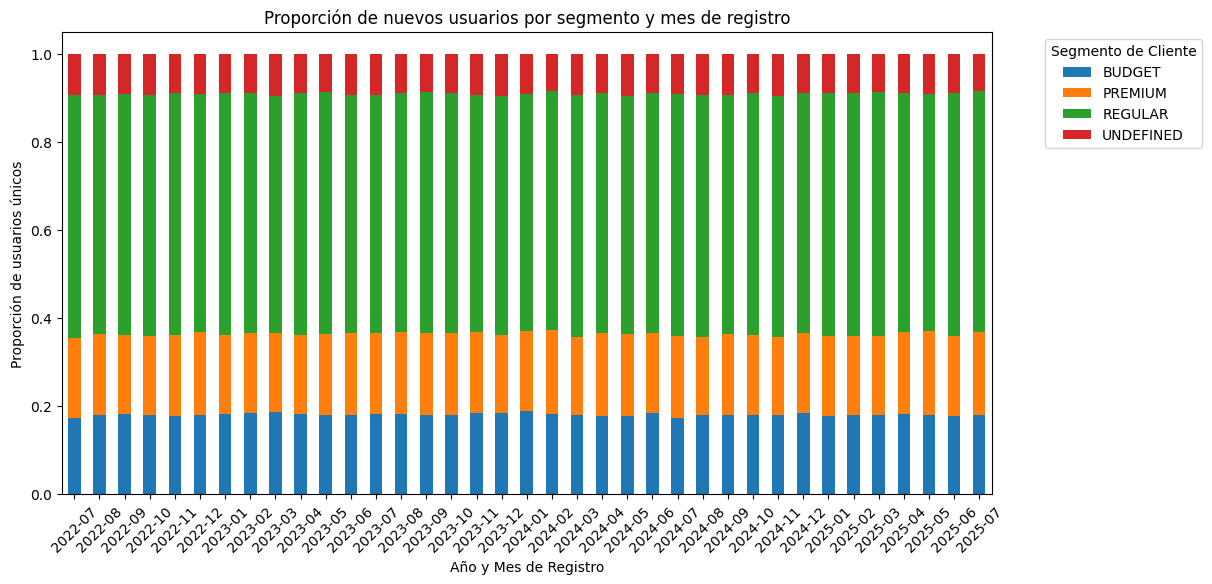
\includegraphics[width=0.8\textwidth]{imagenes/datos_uniformes/proporcion_de_nuevos_usuarios.png}
    \caption{Proporción de nuevos usuarios por segmento y mes de registro}
    \label{fig:proporcion_de_nuevos_usuarios}
\end{figure}

A continuación se muestran dos gráficos que ilustran la cantidad de usuarios por estado. En la figura \ref{fig:usuarios_por_estado} se puede observar que la mayoría de los estados tienen una cantidad similar de usuarios. En esta primera figura se visualiza una escala de 0 a 7000, y vemos que todos los estados tienen colores muy similares.

\begin{figure}[H]
    \centering
    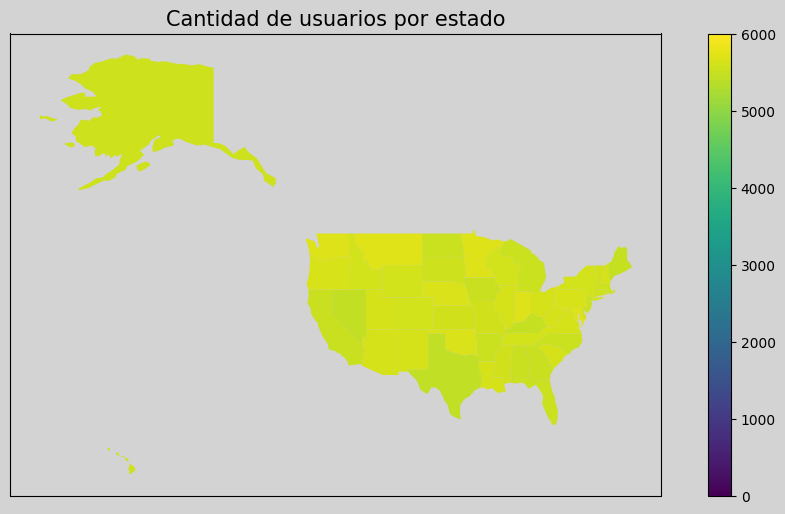
\includegraphics[width=0.8\textwidth]{imagenes/datos_uniformes/usuarios_por_estado.png}
    \caption{Cantidad de usuarios por estado}
    \label{fig:usuarios_por_estado}
\end{figure}

En la figura \ref{fig:usuarios_por_estado_closer} se puede ver el mismo mapa con una escala más cerrada, aproximadamente de 6300 a 6700. En este gráfico sí se pueden notar colores más variados. Aún así hay que notar que la diferencia entre el estado con más usuarios y el estado con menos usuarios es de a lo sumo 400 usuarios, lo cual es una diferencia bastante baja tomando en consideración el total de usuarios por estado. Esto refuerza la idea de que los datos son simulados y no representan una distribución realista de usuarios por estado. Notar como, por ejemplo, el estado de Alaska  tiene muchos más usuarios que Texas, lo cual es muy improbable en un escenario real.

\begin{figure}[H]
    \centering
    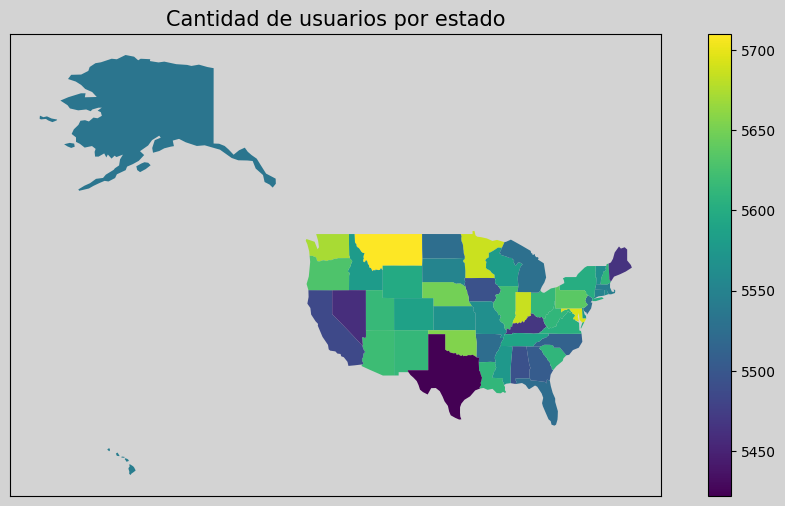
\includegraphics[width=0.8\textwidth]{imagenes/datos_uniformes/usuarios_por_estado_closer.png}
    \caption{Cantidad de usuarios por estado (detalle)}
    \label{fig:usuarios_por_estado_closer}
\end{figure}

\subsection{Órdenes}

En la figura \ref{fig:ordenes_por_estado} se pueden visualizar la cantidad de órdenes totales por estado. Nuevamente, se puede observar que la mayoría de los estados tienen una cantidad similar de órdenes, a excepción de los estados militares de Estados Unidos (AA, AE, AP) que tienen una cantidad considerablemente mayor de órdenes, casi exactamente el doble.

\begin{figure}[H]
    \centering
    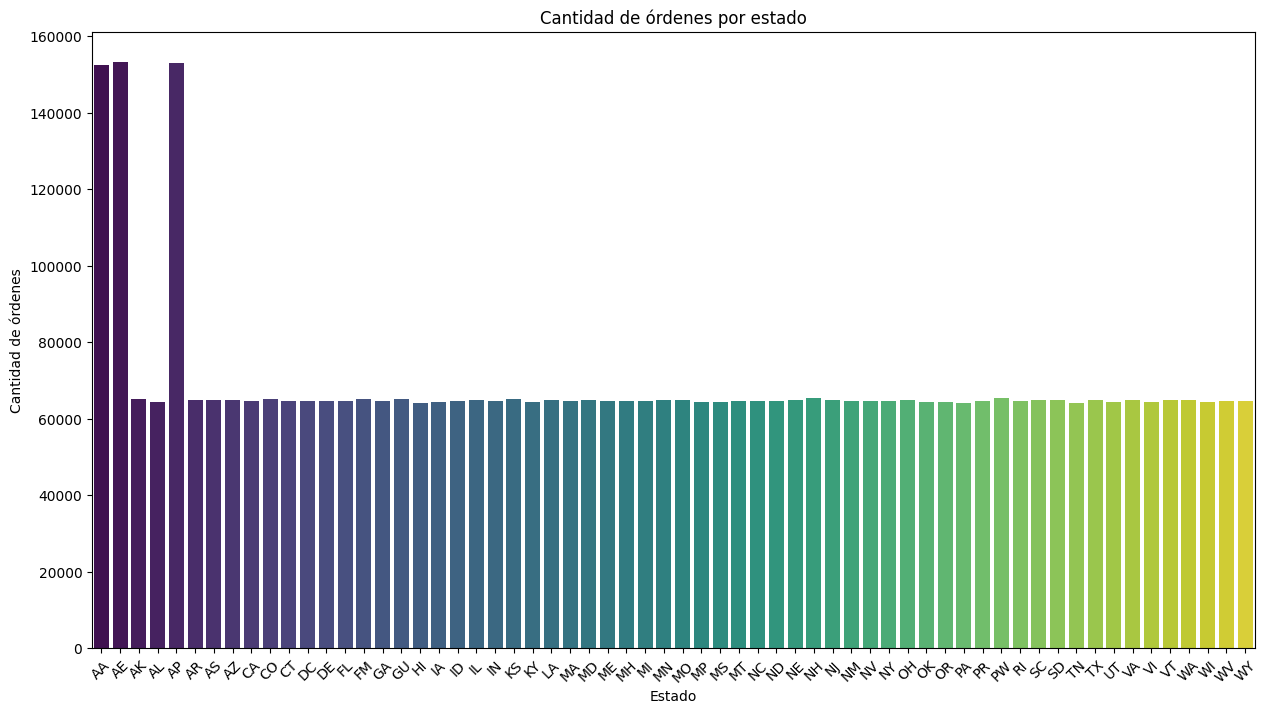
\includegraphics[width=0.8\textwidth]{imagenes/datos_uniformes/ordenes_por_estado.png}
    \caption{Cantidad de órdenes por estado}
    \label{fig:ordenes_por_estado}
\end{figure}

\begin{figure}[H]
    \centering
    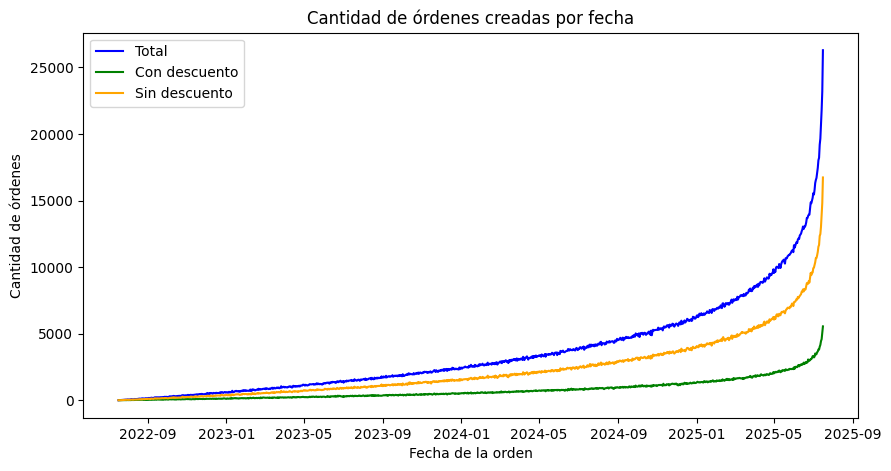
\includegraphics[width=0.8\textwidth]{imagenes/datos_uniformes/cantidad_de_ordenes_por_fecha.png}
    \caption{Cantidad de órdenes por fecha (agrupados con descuento, sin descuento y totales)}
    \label{fig:cantidad_de_ordenes_por_fecha}
\end{figure}

En la figura \ref{fig:cantidad_de_ordenes_por_fecha} se puede observar la cantidad de órdenes por fecha (i.e. la cantidad de filas en la tabla \texttt{orders} por fecha), diferenciados para órdenes con descuento, sin descuento y el total. Se puede observar que las tres curvas siguen una tendencia muy marcada, parecida a una curva exponencial, con desviaciones muy pequeñas. \\
Esto nos da una idea de cómo se pueden haber simulado los datos, podemos inferir que se utilizó algún tipo de función matemática para generar estas cifras y que se utilizó un porcentaje fijo de órdenes con descuento respecto al total de órdenes.

En la figura \ref{fig:ordenes_por_estado_en_el_tiempo} se puede observar la proporción de órdenes por estado en el tiempo. Cada color representa uno de los estados. Se puede observar nuevamente la tendencia muy marcada en todos los estados, con desviaciones muy pequeñas. Se puede apreciar muy bien cómo la cantidad de órdenes por mes es casi idéntica para todos los estados. La única excepción son las cantidades en los estados militares como se vió en la figura \ref{fig:ordenes_por_estado}, que aún puede verse que tienen que siguen una tendencia similar a la de los demás estados.

\begin{figure}[H]
    \centering
    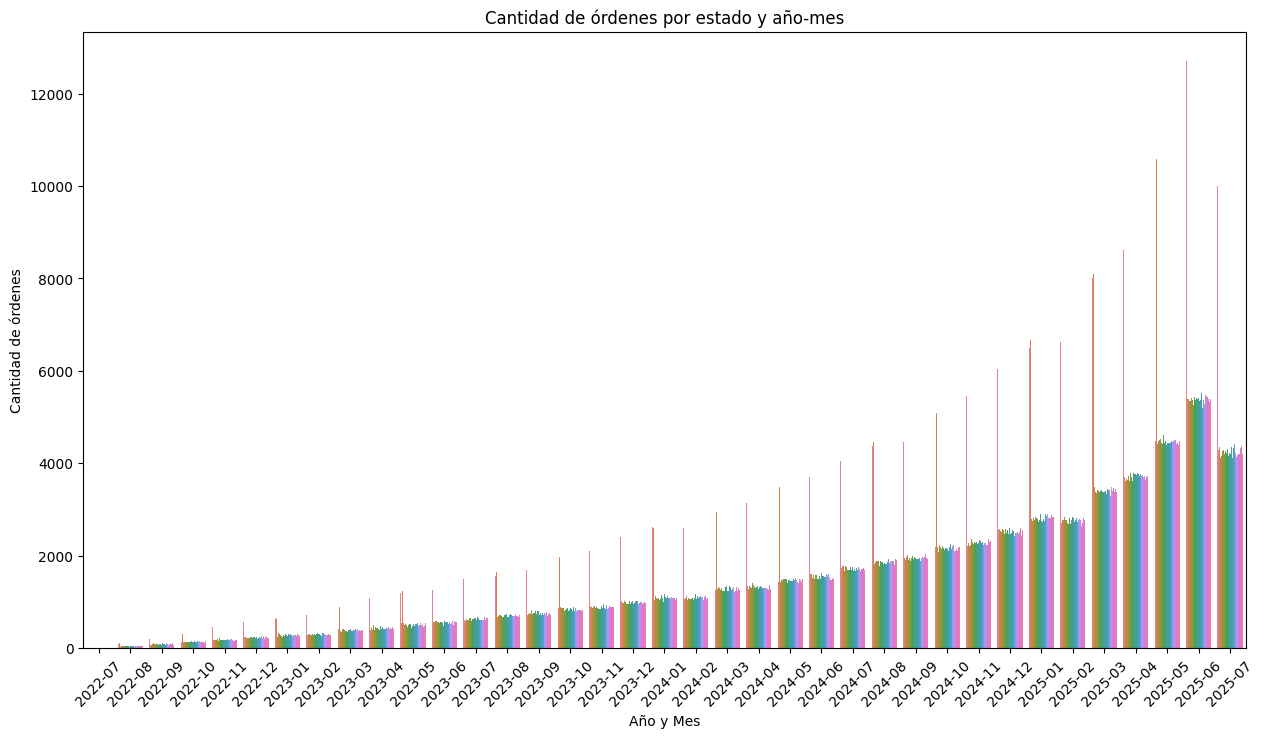
\includegraphics[width=0.8\textwidth]{imagenes/datos_uniformes/ordenes_por_estado_en_el_tiempo.png}
    \caption{Proporción de órdenes por estado en el tiempo}
    \label{fig:ordenes_por_estado_en_el_tiempo}
\end{figure}

La única anomalía en la tendencia que siguen los datos es en el último mes registrado. Esto puede deberse a que los datos fueron generados hasta una fecha específica (17/07/2025) y no se completó el mes, por lo que la cantidad de órdenes en ese mes es considerablemente menor.

\subsection{Inventario}

En la figura \ref{fig:movimientos_por_tipo_y_dia} se puede observar la cantidad de movimientos de inventario por tipo y día. Se puede observar que a lo largo del tiempo se registran cantidades de movimientos similares para cada tipo de movimiento. La única excepción es el tipo de movimiento `Undefined', que tiene una cantidad considerablemente menor de movimientos registrados.

Notar cómo se forman franjas en las cuales se distribuyen los puntos, donde cada uno representa la cantidad de movimientos que hubo en un día. Si los datos fueran reales, se podría esperar ver que las franjas sigan un ciclo anual, con más movimientos en ciertas épocas del año (por ejemplo, en diciembre por las fiestas) y menos en otras. Sin embargo, en este caso las franjas no siguen un patrón anual, sino que parecen estar distribuidas de manera uniforme a lo largo del tiempo.

\begin{figure}[H]
    \centering
    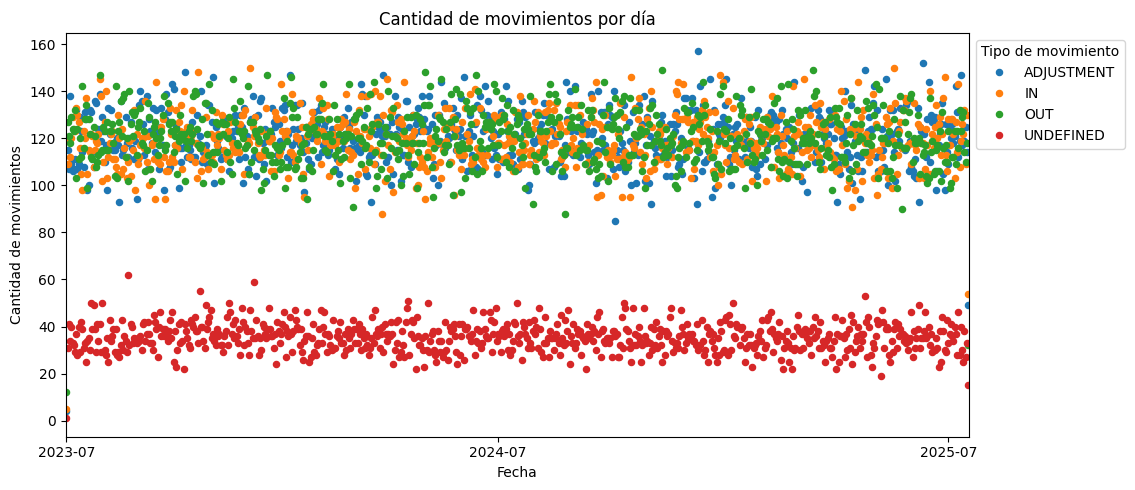
\includegraphics[width=0.8\textwidth]{imagenes/datos_uniformes/movimientos_por_tipo_y_dia.png}
    \caption{Cantidad de movimientos por tipo y día}
    \label{fig:movimientos_por_tipo_y_dia}
\end{figure}

\begin{figure}[H]
    \centering
    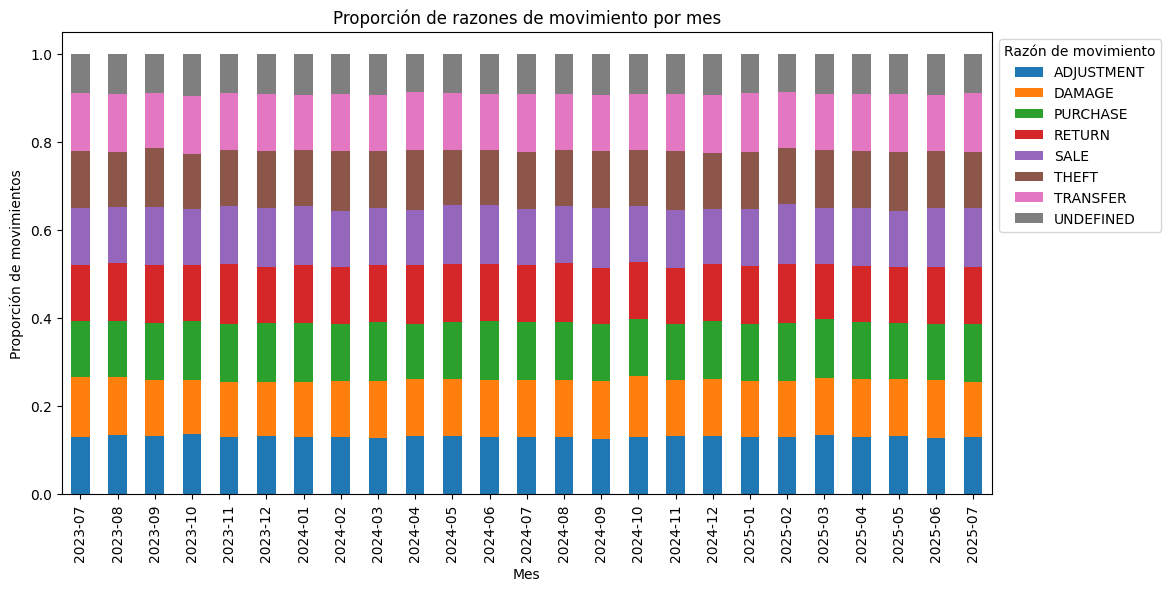
\includegraphics[width=0.8\textwidth]{imagenes/datos_uniformes/razones_de_movimientos.png}
    \caption{Proporción de razones de movimientos por mes}
    \label{fig:razones_de_movimientos}
\end{figure}

En la figura \ref{fig:razones_de_movimientos} nuevamente se puede observar una distribución uniforme en el tiempo, esta vez de las razones de movimientos de inventario. Se puede observar que hay una cantidad muy similar de todos los movimientos, y que la proporción entre ellos se mantiene casi constante a lo largo del tiempo. Por ejemplo podemos ver que la proporción entre movimientos de tipo `Sale' y `Theft' es casi exactamente 1:1 en todos los meses, lo cual sería preocupante en un escenario real.

Finalmente, se presentan dos gráficos que personalmente me gustan mucho. \\
En la figura \ref{fig:cambios_cantidad_mes} se puede observar el cambio acumulado en la cantidad de unidades del inventario (sin diferenciar entre productos). Es notable cómo la línea negra, que representa el cambio total en la cantidad, se mantiene casi constante a lo largo del tiempo, con pequeñas variaciones. Esto indica que la cantidad de unidades en el inventario no varía mucho a lo largo del tiempo. Se puede observar que en todos los meses las cantidades en los movimientos `IN' se compensan con las de los movimientos `OUT', mientras que las cantidades de los movimientos `ADJUSTMENT' y `UNDEFINED' casi no aparecen en el gráfico, lo que indica que las entradas en la tabla se cancelan entre sí en un mismo mes.

Por último, en la figura \ref{fig:distribucion_tipos_de_mov} se puede observar la distribución de los tipos de movimiento en el tiempo. Podemos observar que, aún con una elevada cantidad de \texttt{bins} en el histograma, la distribución de los tipos de movimiento es prácticamente constante para los tipos de movimiento `IN', `OUT' y `ADJUSTMENT'. Además, podemos ver límites muy marcados y redondos en los valores que toma cada tipo de movimiento. \\
También se puede observar que el tipo de movimiento `UNDEFINED' no sigue una distribución uniforme, pero sigue la misma distribución que el total de movimientos. De esta manera podemos inferir que para el dataset se crearon los datos `IN', `OUT' y `ADJUSTMENT' de manera uniforme, y luego los datos `UNDEFINED' se crearon como un porcentaje fijo del total de movimientos.

\begin{figure}[H]
    \centering
    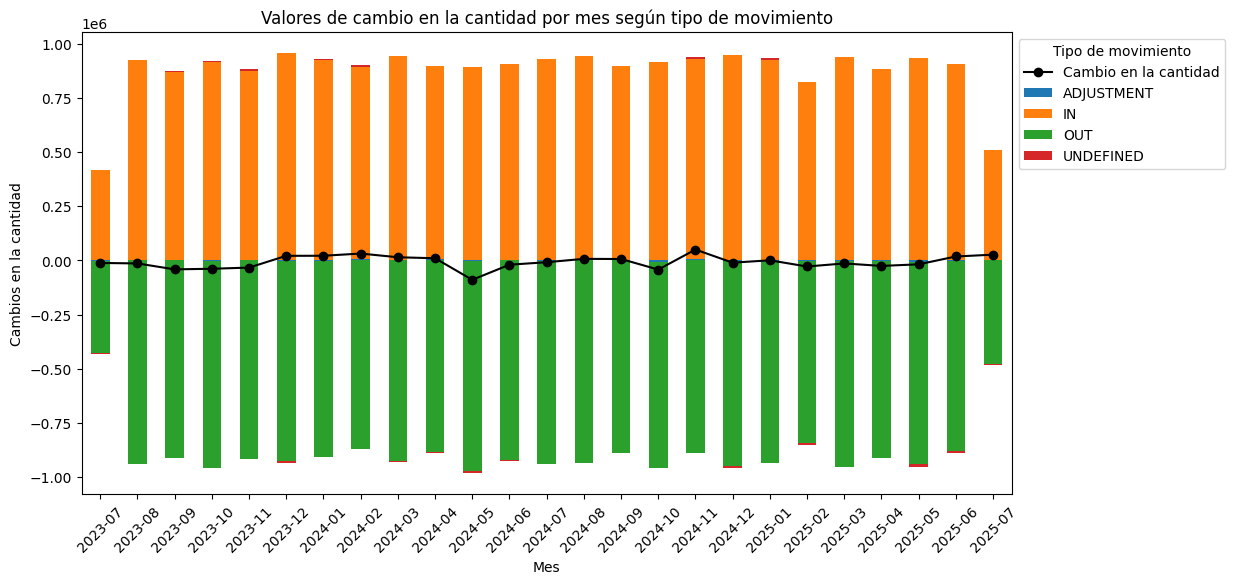
\includegraphics[width=0.8\textwidth]{imagenes/datos_uniformes/cambios_cantidad_mes.png}
    \caption{Valores de cambio en la cantidad por mes según tipo de movimiento}
    \label{fig:cambios_cantidad_mes}
\end{figure}

\begin{figure}[H]
    \centering
    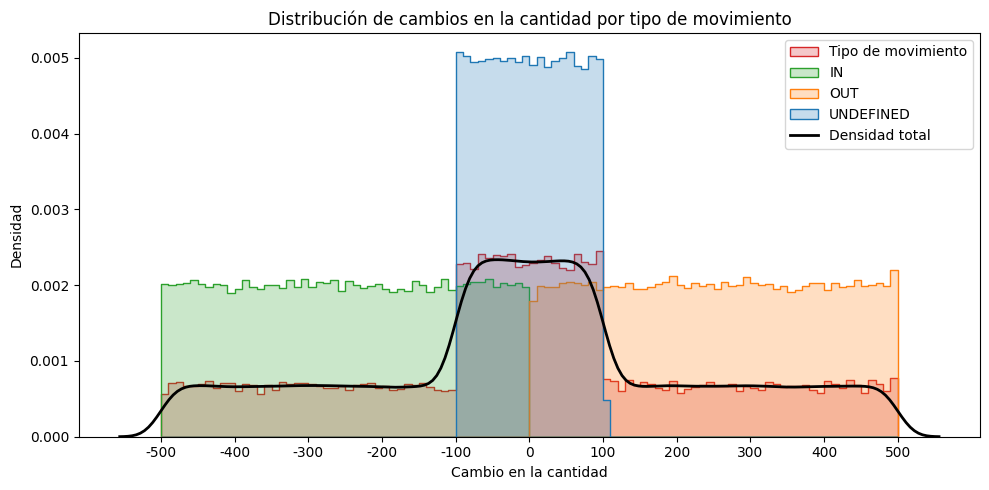
\includegraphics[width=0.8\textwidth]{imagenes/datos_uniformes/distribucion_tipos_de_mov.png}
    \caption{Distribución de valores de cambio en la cantidad según tipo de movimiento}
    \label{fig:distribucion_tipos_de_mov}
\end{figure}